% ===========================================================================
% III. Reputation System Model
% ===========================================================================
\section{Reputation System Model}
\label{sec:sysmodel}

\subsection{Overview}

The target system is a Bayesian Beta-reputation engine deployed as a
Hyperledger Fabric smart contract~\cite{almaayn2024unified}.  It maintains
per-actor reputation scores derived from peer ratings of observed
performance, with economic incentives discouraging dishonest reporting and
access controls preventing privilege escalation.  We summarize the
components modeled in the MARL environment; full implementation details
appear in the companion paper.

\subsection{Bayesian Beta Scoring}

Each actor $i$ maintains a reputation score $\mu_i \in [0,1]$ derived from
a Beta distribution with parameters $(\alpha_i, \beta_i)$:
\begin{equation}
  \mu_i = \frac{\alpha_i}{\alpha_i + \beta_i},
  \label{eq:beta_mean}
\end{equation}
where $\alpha_i$ accumulates positive ratings and $\beta_i$ accumulates
negative ratings.  The mean $\mu_i$ is the point estimate of actor $i$'s
trustworthiness.  To quantify uncertainty, the system reports the Wilson
95\% confidence interval width $w_i$:
\begin{equation}
  w_i = \frac{2z\sqrt{\hat{p}(1-\hat{p}) + z^2/(4n)}}{1 + z^2/n},
  \label{eq:wilson_ci}
\end{equation}
where $\hat{p} = \mu_i$, $n = \alpha_i + \beta_i$, and $z = 1.96$.  Actors
with fewer ratings have wider CIs, making it harder to exploit the system
through sparse identities.

\subsection{Temporal Decay}

To prevent stale ratings from dominating long-term scores, the system
applies exponential decay at each write event:
\begin{equation}
  \alpha_i \leftarrow \alpha_i \cdot \lambda^{\Delta t},\quad
  \beta_i  \leftarrow \beta_i  \cdot \lambda^{\Delta t},
  \label{eq:decay}
\end{equation}
where $\Delta t$ is the elapsed time in days and $\lambda = 0.98$ is the
daily decay factor.  Decay is applied before the new rating is added,
so that recent evidence always dominates.

\subsection{Stake-Based Economic Incentives}

Each agent $i$ holds a stake $s_i \geq 0$, which is at risk when submitting
ratings.  Dishonest ratings — detected with probability $p_d = 0.85$ by
cross-validator comparison — result in stake slashing: $s_i \leftarrow
s_i - \delta_s$, where $\delta_s$ is a configurable penalty.  Agents
with insufficient stake ($s_i < s_{\min}$) cannot submit ratings, creating
an economic entry barrier for Sybil identities.

\subsection{Defense Mechanisms}

The system implements the following layered defenses, which are modeled
as action-conditional reward signals in the MARL environment:

\begin{itemize}[noitemsep]
  \item \textbf{Self-rating detection} (action 7): Deterministic check;
        submitting a rating for one's own identity triggers a reward penalty
        of $-5.0$ and the rating is rejected.
  \item \textbf{Administrative escalation} (action 8): Unauthorized attempts
        to invoke admin-only functions (e.g., \icode{SetReputationGate},
        \icode{AddAdmin}) receive penalty $-5.0$ and are blocked.
  \item \textbf{Evidence tampering} (action 9): Off-chain audit with
        probabilistic detection; tampered submissions are flagged with
        probability $p = 0.80$, incurring penalty $-2.0$ on detection.
  \item \textbf{Reputation-gate bypass} (action 10): Attempts to invoke
        gate-protected functions without meeting the threshold score are
        rejected with penalty $-3.0$.
  \item \textbf{Provenance replay} (action 11): Duplicate transaction IDs
        detected by ledger lookup; replays receive penalty $-5.0$ and
        are rejected.
  \item \textbf{Sybil flooding} (action 5): Sybil identities are permitted
        but their CI widths grow faster than real identities, limiting their
        amplification power.  Honest agents receive a defense dividend of
        $+0.1$ per blocked Sybil action.
  \item \textbf{Collusion rings} (actions 1--4 within group): Coordinated
        positive ratings among colluding agents are partially detected via
        meta-reputation weighting; CI widening limits score amplification.
\end{itemize}

\subsection{Threat Model}

We consider adversarial agents with:
\begin{itemize}[noitemsep]
  \item Full knowledge of the action space and reward structure (white-box).
  \item The ability to submit any of the 12 actions each turn, including all
        attack-class actions.
  \item An additional reward bonus $b \in [0.5, 2.0]$ per successful dishonest
        action, representing economic motivation beyond reputation gain.
\end{itemize}
We do not consider attacks requiring out-of-band communication channel
compromise (e.g., private key theft) or consensus-layer attacks on the
blockchain itself.  The objective is to evaluate whether the application-layer
incentive structure is sufficient to deter rational adversaries.

\begin{figure}[!t]
  \centering
  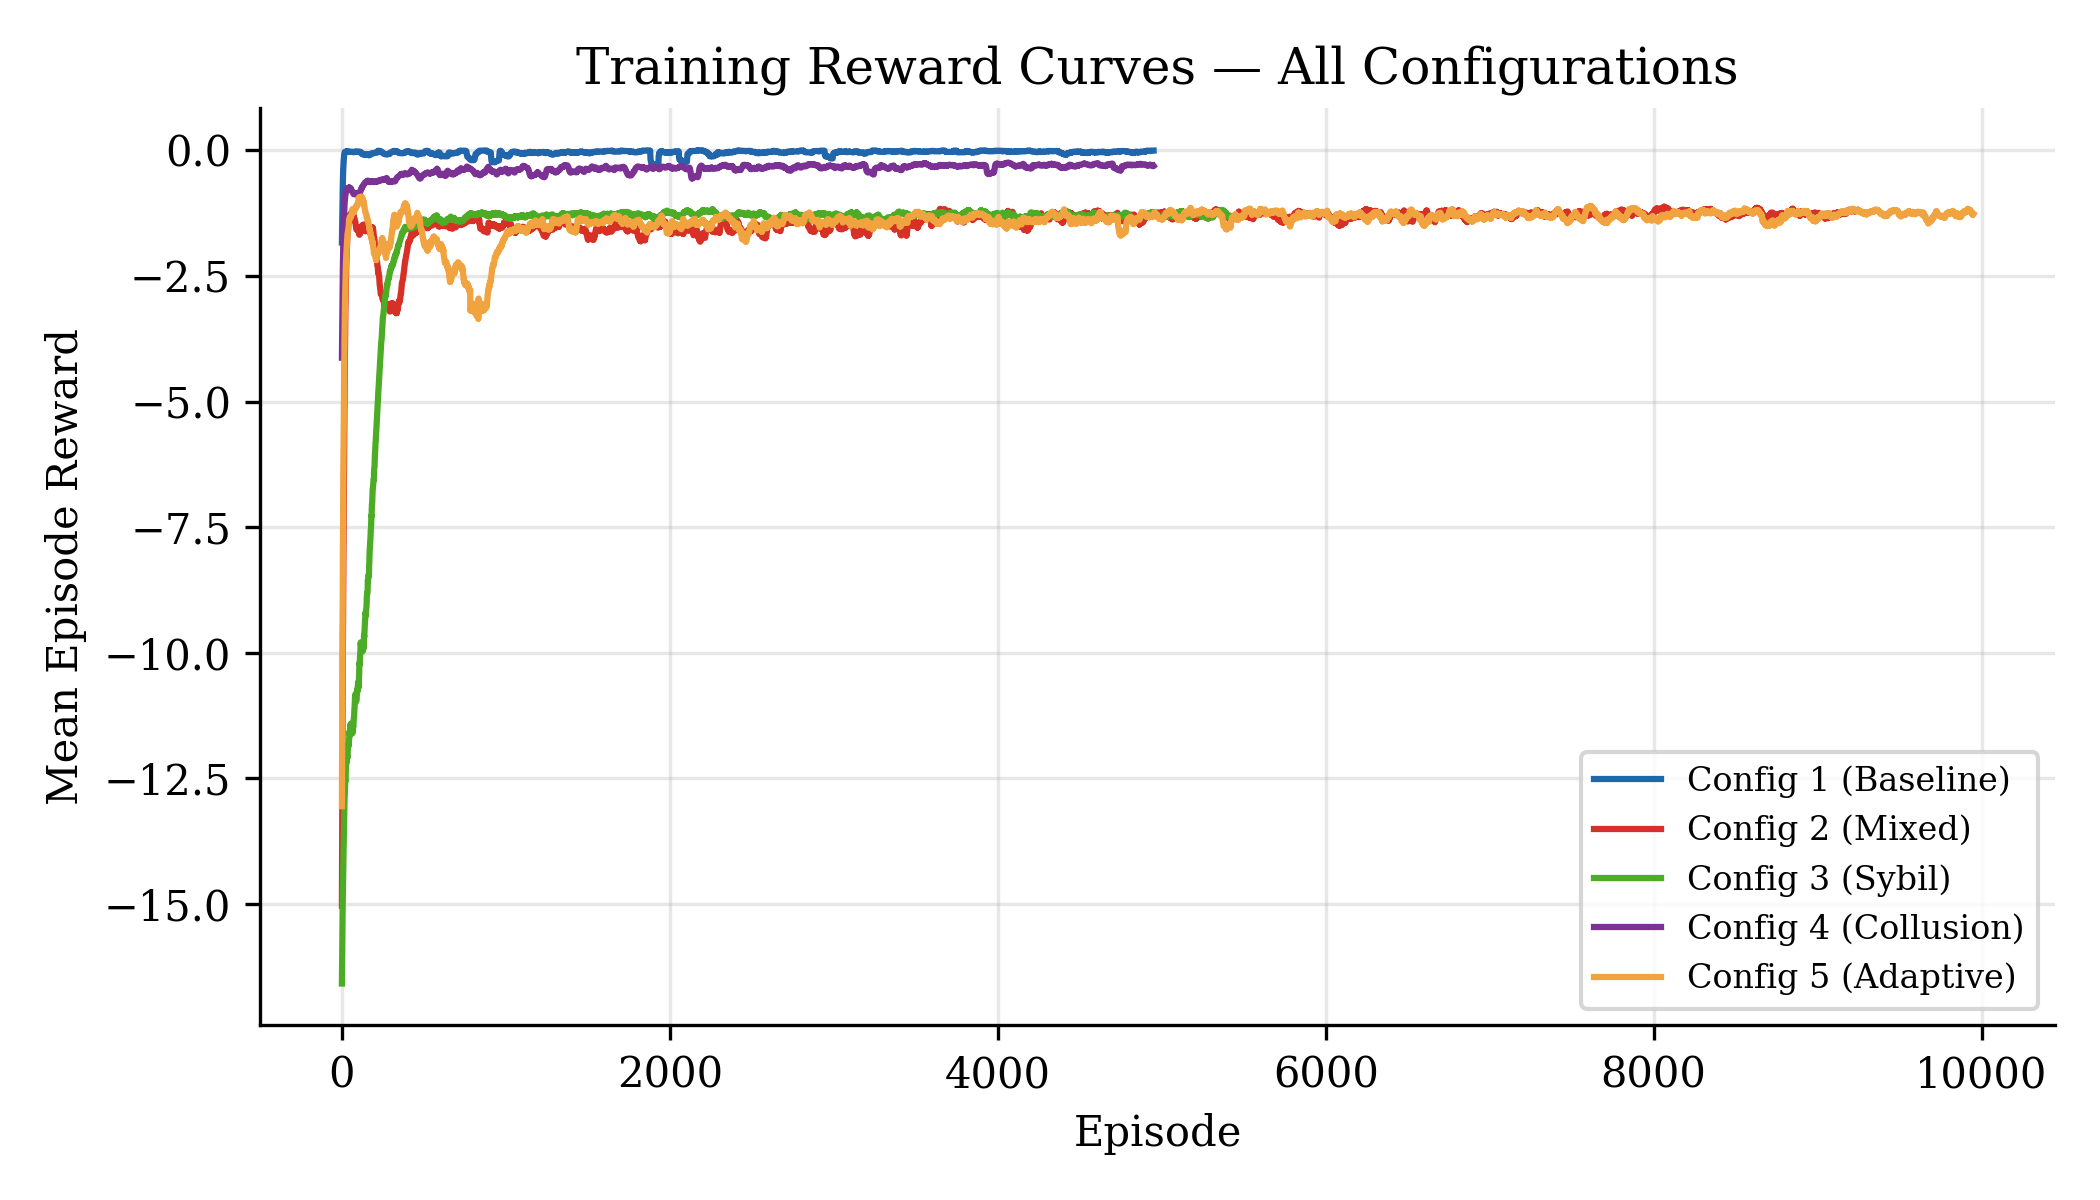
\includegraphics[width=0.9\columnwidth]{figures/fig_training_curves.png}
  \caption{Training reward curves for all 11 experimental configurations
           (mean $\pm$ std across 5 seeds).  Honest baseline (C1) converges
           to near-zero reward within 2{,}000 episodes; single-attack configs
           (C6--C10) converge within 3{,}000--5{,}000 episodes; the
           comprehensive config (C11) shows high variance throughout.}
  \label{fig:training_curves}
\end{figure}
